\begin{frame}[shrink=8]
    \frametitle{Traffic light modeling}
    \metroset{block=fill}
    \uncover<1->{
    \begin{block}{Two level of complexity}
    \begin{itemize}
    \item Size of the network's model
    \item Traffic light almost each intersection
    \end{itemize}
    \end{block}
    }
    \begin{columns}
    \column{0.45\textwidth}
    \uncover<2->{
    \begin{block}{Piece--wise system representation}
    \begin{center}
    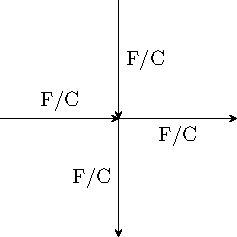
\includegraphics[scale=0.55]{fig_46_intersection}
    \end{center}
    CTM still possible (each road is a cell) but the choice Free/Congested can give dimensional problem ($\sim 2^{\symbol{35}\mbox{roads}}$)
    \end{block}
    }
    \column{0.45\textwidth}
    \uncover<3->{
    \begin{block}{Discontinuities in traffic signal}
    \begin{center}
    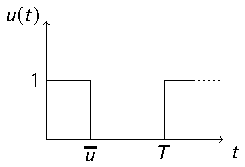
\includegraphics[scale=0.65]{fig_47_light-plot}
    \end{center}
    A traffic light is a $T$--periodic, discontinuous signal $u(t)\in\{{\color{red}0},{\color{green}1}\}$, with duty cycle $\frac{1}{T}\int_0^T u(t) \onslide<2->{ = \frac{\overline{u}}{T}}$
    \end{block}
    }
    \end{columns}
\end{frame}